\documentclass[a4paper,10pt,foldmark,notumble]{leaflet}

% Compile with XeLaTeX!!!
\usepackage{ifxetex}
\ifxetex
\pdfpagewidth=3\paperwidth
\pdfpageheight=\paperheight
\usepackage{fontspec}
\defaultfontfeatures{Mapping=tex-text}
\input{UBScala/fontspec}
\setmainfont{UBScala}
\setsansfont{UBScalaSans}
\else
\fi

\usepackage[dvipsnames,usenames]{xcolor}
%%UNIBA-Colors
\definecolor{unibablueI}{HTML}{00457D}
\definecolor{unibablueII}{HTML}{336A97}
\definecolor{unibablueIII}{HTML}{6690B1}
\definecolor{unibablueIV}{HTML}{99B5CB}
\definecolor{unibablueV}{HTML}{CCDAE5}

\definecolor{unibayellowI}{HTML}{FFD300}
\definecolor{unibayellowII}{HTML}{FFDC33}
\definecolor{unibayellowIII}{HTML}{FFE566}
\definecolor{unibayellowIV}{HTML}{FFED99}
\definecolor{unibayellowV}{HTML}{FFF6CC}

\definecolor{unibagreenI}{HTML}{97BF0D}
\definecolor{unibagreenII}{HTML}{ACCC3D}
\definecolor{unibagreenIII}{HTML}{C1D86E}
\definecolor{unibagreenIV}{HTML}{D5E59E}
\definecolor{unibagreenV}{HTML}{EAF2CF}
%Not CD, darker versions
\definecolor{nounibagreenI}{HTML}{82A50B}
\definecolor{nounibagreenII}{HTML}{708C0A}

\definecolor{unibaredI}{HTML}{E6444F}
\definecolor{unibaredII}{HTML}{EB6972}
\definecolor{unibaredIII}{HTML}{F08F95}
\definecolor{unibaredIV}{HTML}{F5B4B8}
\definecolor{unibaredV}{HTML}{FADADC}
%Not CD, darker versions
\definecolor{nounibaredI}{HTML}{CC3D47}
\definecolor{nounibaredII}{HTML}{B3363E}

\definecolor{unibagrayI}{HTML}{878783}
\definecolor{unibagrayII}{HTML}{9F9F9C}
\definecolor{unibagrayIII}{HTML}{B7B7B5}
\definecolor{unibagrayIV}{HTML}{CFCFCE}
\definecolor{unibagrayV}{HTML}{E7E7E6}

%%%%%%%%%%%%%%%%%%%%%%%%%%%%%%%%%%%%%%%%%%%%%%%%%%%%%%%%%%%
% TIKZ Configuration
%%%%%%%%%%%%%%%%%%%%%%%%%%%%%%%%%%%%%%%%%%%%%%%%%%%%%%%%%%%
\usepackage{tikz}
\usetikzlibrary{positioning,patterns,calc}


\renewcommand*\foldmarkrule{.3mm}
\renewcommand*\foldmarklength{5mm}

\usepackage{amsmath}
%\usepackage[T1]{fontenc}
\usepackage{textcomp}
\usepackage{mathptmx}
%\usepackage[scaled=0.9]{helvet}
\makeatletter
\def\ptmTeX{T\kern-.1667em\lower.5ex\hbox{E}\kern-.075emX\@}
\DeclareRobustCommand{\ptmLaTeX}{L\kern-.3em
        {\setbox0\hbox{T}%
         %\vb@xt@ % :-)
         \vbox to\ht0{\hbox{%
                            \csname S@\f@size\endcsname
                            \fontsize\sf@size\z@
                            \math@fontsfalse\selectfont
                            A}%
                      \vss}%
        }%
        \kern-.12em
        \ptmTeX}
\makeatother
%\let\TeX=\ptmTeX
%\let\LaTeX=\ptmLaTeX
\usepackage{shortvrb}
%\MakeShortVerb{\|}
\usepackage{url}
\usepackage{graphicx}
\usepackage{longtable}
\usepackage{colortbl}
\usepackage{multirow,varwidth,array}
\definecolor{LIGHTGRAY}{gray}{.9}

%%%%\renewcommand{\descfont}{\normalfont}
\newcommand\Lpack[1]{\textsf{#1}}
\newcommand\Lclass[1]{\textsf{#1}}
\newcommand\Lopt[1]{\texttt{#1}}
\newcommand\Lprog[1]{\textit{#1}}

\newcommand*\defaultmarker{\textsuperscript\textasteriskcentered}

%\usepackage[colorlinks=true, urlcolor=unibablueI]{hyperref}

\title{\bf MMB \& DFT 2014}

\author{%
\Large \bf University of Bamberg
%  Martin Schmoll\\
%  Predrag Puno\v{s}evac
}
\date{\bf March 17 -- 19, 2014 }

\CutLine*{1}
\CutLine*{6}

%\AddToBackground{1}{%  Background of a small page
%  \put(0,0){\textcolor{Cerulean}{\rule{\paperwidth}{\paperheight}}}}


%\AddToBackground{1}{%  Background of a small page
%  \put(115,530){\includegraphics[scale=0.12]{tiger.eps}}}


\AddToBackground{6}{%  Background of a small page
  \put(0,0){\textcolor{unibablueV}{\rule{\paperwidth}{\paperheight}}}}


%\AddToBackground*{2}{% Background of a large page
%  \put(\LenToUnit{.5\paperwidth},\LenToUnit{.5\paperheight}){%
%    \makebox(0,0)[c]{%
%      \resizebox{.9\paperwidth}{!}{\rotatebox{35.26}{%
%        \textsf{\textbf{\textcolor{LIGHTGRAY}{CLEMSON}}}}}}}}


\begin{document}
\maketitle

\newpage
\section{Time Table}

\newcommand{\daywidth}{24mm}
\newcommand{\daytextwidth}{21mm}

\newcommand{\hourseparation}{3mm}

\begin{tikzpicture}[yscale=-0.1, xscale=0.1, node distance=1mm,outer sep = 0pt]

% Style for Days
\tikzstyle{day}=[draw, white, rectangle,  minimum height=5mm, minimum width=\daywidth, fill=unibablueI,anchor=north west, align=center, font=\small]
% Style for hours
\tikzstyle{hour}=[draw, rectangle, minimum height=5mm, minimum width=8mm, fill=unibagrayIV, anchor=north west, align=center, font=\scriptsize]

\tikzstyle{default}=[anchor=north west,draw=red]

% Styles for events
% Duration of sequences
\tikzstyle{hours}=[rectangle,draw, minimum width=\daywidth, text width=\daytextwidth, anchor=north west, align=center, font=\footnotesize]
\tikzstyle{hhours}=[rectangle,draw, minimum width=.5*\daywidth-1.5mm, text width=.5*\daytextwidth-1.5mm, anchor=north west, align=center, font=\footnotesize]

\tikzset{grid/.style={gray,very thin,opacity=1}}

%\node[default] at (-7,-12) {
%        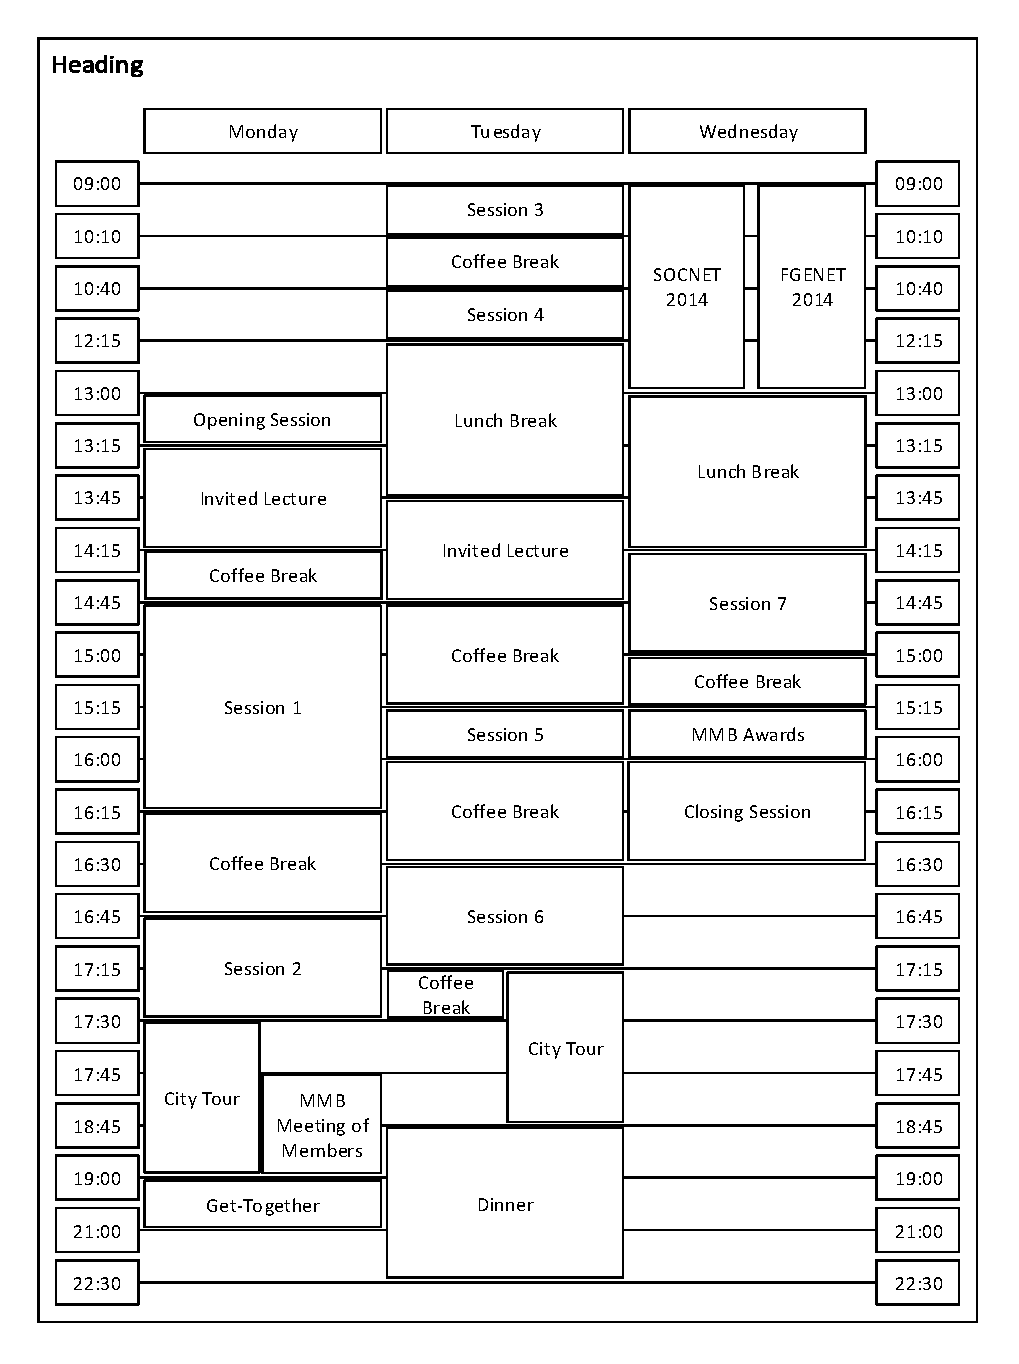
\includegraphics[width=2cm+\textwidth]{images/timetable.pdf}
%    };
    
%\draw[grid] (0,0) grid (10*\textwidth,10*\textheight);

\node[day] (mo) at (9,0) {Monday};
\node[day] (tu) [right = of mo] {Tuesday};
\node[day] (we) [right = of tu] {Wednesday};

\node[hour] (0900) at (0,7) {09:00};
\node[hour] (1010) [below = \hourseparation of 0900] {10:10};
\node[hour] (1040) [below = \hourseparation of 1010] {10:40};
\node[hour] (1215) [below = \hourseparation of 1040] {12:15};
\node[hour] (1300) [below = \hourseparation of 1215] {13:00};
\node[hour] (1315) [below = \hourseparation of 1300] {13:15};
\node[hour] (1345) [below = \hourseparation of 1315] {13:45};
\node[hour] (1415) [below = \hourseparation of 1345] {14:15};
\node[hour] (1445) [below = \hourseparation of 1415] {14:45};
\node[hour] (1500) [below = \hourseparation of 1445] {15:00};
\node[hour] (1515) [below = \hourseparation of 1500] {15:15};
\node[hour] (1600) [below = \hourseparation of 1515] {16:00};
\node[hour] (1615) [below = \hourseparation of 1600] {16:15};
\node[hour] (1630) [below = \hourseparation of 1615] {16:30};
\node[hour] (1645) [below = \hourseparation of 1630] {16:45};
\node[hour] (1715) [below = \hourseparation of 1645] {17:15};
\node[hour] (1730) [below = \hourseparation of 1715] {17:30};
\node[hour] (1745) [below = \hourseparation of 1730] {17:45};
\node[hour] (1845) [below = \hourseparation of 1745] {18:45};
\node[hour] (1900) [below = \hourseparation of 1845] {19:00};
\node[hour] (2100) [below = \hourseparation of 1900] {21:00};
\node[hour] (2230) [below = \hourseparation of 2100] {22:30};

% Monday
\node[hours, minimum height = 7mm, fill=white] (os) at($(1300.west)+(mo.north west)+(0,.5)$) {Opening Session};
\node[hours, minimum height = 15mm, fill=unibayellowV] (il1) [below = of os] {Invited Lecture\\ S{\o}ren Asmussen};
\node[hours, minimum height = 7mm, fill=white] (cb1) [below = of il1] {Coffee Break};
\node[hours, minimum height = 31mm, fill=unibablueV] (s1) [below = of cb1] {Session 1};
\node[hours, minimum height = 15mm, fill=white] (cb2) [below = of s1] {Coffee Break};
\node[hours, minimum height = 15mm, fill=unibablueV] (s2) [below = of cb2] {Session 2};
% night program
\node[hhours, minimum height = 23mm, fill=white] (ct1) at($(1730.west)+(mo.north west)+(0,.5)$) {City Tour};
\node[hhours, minimum height = 15mm, fill=white] (mom) at($(1745.west)+(mo.north west)+(12.5,.5)$) {\tiny MMB Meeting of Members};
\node[hours, minimum height = 7mm, fill=white] (gt) at($(1900.west)+(mo.north west)+(0,.5)$) {Get-Together};

% Tuesday
\node[hours, minimum height = 7mm, fill=unibablueV] (s3) at($(0900.west)+(tu.north west)+(0,.5)$) {Session 3};
\node[hours, minimum height = 7mm, fill=white] (cb3) [below = of s3] {Coffee Break};
\node[hours, minimum height = 7mm, fill=unibablueV] (s4) [below = of cb3] {Session 4};
\node[hours, minimum height = 23mm, fill=white] (lb1) [below = of s4] {Lunch Break};
\node[hours, minimum height = 15mm, fill=unibayellowV] (il2) [below = of lb1] {Invited Lecture\\ James Roberts};
\node[hours, minimum height = 15mm, fill=white] (cb4) [below = of il2] {Coffee Break};
\node[hours, minimum height = 7mm, fill=unibablueV] (s5) [below = of cb4] {Session 5};
\node[hours, minimum height = 15mm, fill=white] (cb5) [below = of s5] {Coffee Break};
\node[hours, minimum height = 15mm, fill=unibagrayV] (s6) [below = of cb5] {Session 6};
% night program
\node[hhours, minimum height = 23mm, fill=white] (ct2) at($(1715.west)+(tu.north west)+(0,.5)$) {City Tour};
\node[hhours, minimum height = 7mm, fill=white] (cb6) at($(1715.west)+(tu.north west)+(12.5,.5)$) {\scriptsize Coffee Break};
\node[hours, minimum height = 23mm, fill=white] (di) at($(1845.west)+(tu.north west)+(0,.5)$) {Dinner};

% Wednesday
%\node[hhours, minimum height = 31mm, fill=white] (so) at($(0900.west)+(we.north west)+(0,.5)$) {\scriptsize SOCNET 2014};
%\node[hhours, minimum height = 31mm, fill=white] (fg) at($(0900.west)+(we.north west)+(12.5,.5)$) {\scriptsize FGENET 2014};
\node[hours, minimum height = 31mm, fill=unibagreenV] (so) at($(0900.west)+(we.north west)+(0,.5)$) {\footnotesize Workshops\\[3ex] \footnotesize SOCNET\\[1ex] \footnotesize FGENET\\[1ex] \footnotesize WoNeCa (-- 16:00)};
\node[hours, minimum height = 23mm, fill=white] (lb2) at($(1300.west)+(we.north west)+(0,.5)$) {Lunch Break};
\node[hours, minimum height = 15mm, fill=unibablueV] (s7) [below = of lb2] {Session 7};
\node[hours, minimum height = 7mm, fill=white] (cb7) [below = of s7] {Coffee Break};
\node[hours, minimum height = 7mm, fill=white] (ma) [below = of cb7] {MMB Awards};
\node[hours, minimum height = 15mm, fill=white] (cs) [below = of ma] {Closing Session};
\end{tikzpicture}

\newpage
% TimeTables
\section{Sessions}
\footnotesize

\newcommand\VertEntry[1]{%
  \multirow{3}*{%
    \begin{varwidth}{2em}% --- or minipage, if you prefer a fixed width
    \centering #1%
    \end{varwidth}}}

\begin{longtable}{|p{2em}|p{5.5cm}|p{1cm}|}
\hline
\rowcolor{unibayellowV} \textcolor{unibablueI}{\textbf{MON}} & \textcolor{unibablueI}{\textbf{Invited Lecture}} & \textcolor{unibablueI}{\textbf{Room}}\\
\hline
\endhead
\VertEntry{13:15 \qquad\quad $\vert$ \qquad 14:15} & \multicolumn{2}{p{6.5cm}|}{\textbf{S{\o}ren Asmussen}:} \\
 & \multicolumn{2}{p{6.5cm}|}{Probabilistic Analysis of the RESTART Protocol and Checkpointing in Computer Reliability} \\
 \hline
\end{longtable}
\vspace{-2em}
\begin{longtable}{|p{2em}|p{5.5cm}|p{1cm}|}
\hline
\rowcolor{unibablueV} \textcolor{unibablueI}{\textbf{MON}} & \textcolor{unibablueI}{\textbf{Session 1: "Traffic Modeling, Inference and Estimation" Chair: TODO}} & \textcolor{unibablueI}{\textbf{Room}}\\
\hline
\endhead
 & \multicolumn{2}{p{6.5cm}|}{\textbf{J. Kriege and P. Buchholz}:} \\
 & \multicolumn{2}{p{6.5cm}|}{PH and MAP Fitting with Aggregated Traffic Traces} \\
 \cline{2-3}
\VertEntry{14:40 \qquad\quad $\vert$ \qquad 16:10} & \multicolumn{2}{p{6.5cm}|}{\textbf{N. and U.R. Krieger}:} \\
 & \multicolumn{2}{p{6.5cm}|}{Modeling of Loss Processes Arising from Packet Flows at Bottleneck Links} \\
  \cline{2-3}
 & \multicolumn{2}{p{6.5cm}|}{\textbf{J. Flohr and J. Charzinski}:} \\
 & \multicolumn{2}{p{6.5cm}|}{A Comparative Study of Traffic Properties for Web Pages Optimized for Mobile Hand-Held and Non-Mobile Devices} \\
 \hline
\end{longtable}
\vspace{-2em}
\begin{longtable}{|p{2em}|p{5.5cm}|p{1cm}|}
\hline
\rowcolor{unibablueV} \textcolor{unibablueI}{\textbf{MON}} & \textcolor{unibablueI}{\textbf{Session 2: "Modeling and Analysis Techniques" Chair: TODO}} & \textcolor{unibablueI}{\textbf{Room}}\\
\hline
\endhead
 & \multicolumn{2}{p{6.5cm}|}{\textbf{R. Berndt, P. Bazan, K. Hielscher and R. German}:} \\
\VertEntry{16:45 \qquad\quad $\vert$ \qquad 17:30} & \multicolumn{2}{p{6.5cm}|}{Construction Methods for MDD-based State Space Representations of Unstructured Systems} \\
 \cline{2-3}
 & \multicolumn{2}{p{6.5cm}|}{\textbf{J. Katoen, T. Noll, T. Santen, D. Seifert and H. Wu}:} \\
 & \multicolumn{2}{p{6.5cm}|}{Performance Analysis of Computing Servers - A Case Study Exploiting a New GSPN Semantics} \\
 \hline
\end{longtable}
\vspace{-2em}
\begin{longtable}{|p{2em}|p{5.5cm}|p{1cm}|}
\hline
\rowcolor{unibablueV} \textcolor{unibablueI}{\textbf{TUE}} & \textcolor{unibablueI}{\textbf{Session 3: "Wireless Networks" Chair: TODO}} & \textcolor{unibablueI}{\textbf{Room}}\\
\hline
\endhead
 & \multicolumn{2}{p{6.5cm}|}{\textbf{R. Krenzler and H. Daduna}:} \\
 & \multicolumn{2}{p{6.5cm}|}{Modeling and Performance Analysis of a Node in Delay Tolerant Wireless Sensor Networks} \\
 \cline{2-3}
\VertEntry{09:00 \qquad\quad $\vert$ \qquad 10:10} & \multicolumn{2}{p{6.5cm}|}{\textbf{A. Dittrich, B. Lichtblau, R. Rezende and M. Malek}:} \\
 & \multicolumn{2}{p{6.5cm}|}{Modeling Responsiveness of Decentralized Service Discovery in Wireless Mesh Networks} \\
 \cline{2-3}
 & \multicolumn{2}{p{6.5cm}|}{\textbf{P. Eittenberger and U.R. Krieger}:} \\
 & \multicolumn{2}{p{6.5cm}|}{Performance Evaluation of Forward-Error Correction Mechanisms For Android Devices Based on Raptor Codes} \\
 \hline
\end{longtable}
\vspace{-2em}
\begin{longtable}{|p{2em}|p{5.5cm}|p{1cm}|}
\hline
\rowcolor{unibablueV} \textcolor{unibablueI}{\textbf{TUE}} & \textcolor{unibablueI}{\textbf{Session 4: "Monitoring and Analysis of Protocols and Service Architectures" Chair: TODO}} & \textcolor{unibablueI}{\textbf{Room}}\\
\hline
\endhead
 & \multicolumn{2}{p{6.5cm}|}{\textbf{G. Hasslinger and K. Ntougias}:} \\
 & \multicolumn{2}{p{6.5cm}|}{Evaluation of Caching Strategies based on Access Statistics on Past Requests} \\
 \cline{2-3}
 & \multicolumn{2}{p{6.5cm}|}{\textbf{T. Ho\ss feld, R. Schatz and U.R. Krieger}:} \\
\VertEntry{10:40 \qquad\quad $\vert$ \qquad 12:15} & \multicolumn{2}{p{6.5cm}|}{QoE of YouTube Video Streaming for Current Internet Transport Protocols} \\
 \cline{2-3}
 & \multicolumn{2}{p{6.5cm}|}{\textbf{V. Burger, M. Hirth, C. Schwartz, T. Ho\ss feld and P. Tran-Gia}:} \\
 & \multicolumn{2}{p{6.5cm}|}{Increasing the Coverage of Vantage Points in Distributed Active Network Measurements by Crowdsourcing} \\
  \cline{2-3}
 & \multicolumn{2}{p{6.5cm}|}{\textbf{P. Zwickl, P. Reichl and A. Sackl}:} \\
 & \multicolumn{2}{p{6.5cm}|}{The 15 Commandments of Market Entrance Pricing for Differentiatied Network Services} \\
 \hline
\end{longtable}
\vspace{-2em}
\begin{longtable}{|p{2em}|p{5.5cm}|p{1cm}|}
\hline
\rowcolor{unibayellowV} \textcolor{unibablueI}{\textbf{TUE}} & \textcolor{unibablueI}{\textbf{Invited Lecture}} & \textcolor{unibablueI}{\textbf{Room}}\\
\hline
\endhead
\VertEntry{13:45 \qquad\quad $\vert$ \qquad 14:45} & \multicolumn{2}{p{6.5cm}|}{\textbf{James Roberts}:} \\
 & \multicolumn{2}{p{6.5cm}|}{On the Performance of Caching in Information-centric Networks} \\
 \hline
\end{longtable}
\vspace{-2em}
\begin{longtable}{|p{2em}|p{5.5cm}|p{1cm}|}
\hline
\rowcolor{unibablueV} \textcolor{unibablueI}{\textbf{TUE}} & \textcolor{unibablueI}{\textbf{Session 5: "Reliable Software: Analysis and Testing" Chair: TODO}} & \textcolor{unibablueI}{\textbf{Room}}\\
\hline
\endhead
 & \multicolumn{2}{p{6.5cm}|}{\textbf{S. Kerschbaum, K. Hielscher, R. German and U. Klehmet}:} \\
\VertEntry{15:15 \qquad\quad $\vert$ \qquad 16:00} & \multicolumn{2}{p{6.5cm}|}{A Framework for Establishing Performance Gukarantees in Industrial Automation Networks} \\
 \cline{2-3}
 & \multicolumn{2}{p{6.5cm}|}{\textbf{M. Meitner and F. Saglietti}:} \\
 & \multicolumn{2}{p{6.5cm}|}{Target-Specific Adaptations of Coupling-Based Software Reliability Testing} \\
 \hline
\end{longtable}
\vspace{-2em}
\begin{longtable}{|p{2em}|p{5.5cm}|p{1cm}|}
\hline
\rowcolor{unibagrayV} \textcolor{unibablueI}{\textbf{TUE}} & \textcolor{unibablueI}{\textbf{Session 6: "Tools" Chair: TODO}} & \textcolor{unibablueI}{\textbf{Room}}\\
\hline
\endhead
 & \multicolumn{2}{p{6.5cm}|}{\textbf{A. Gouberman, M. Riedl, M. Siegle and C. Grand}:} \\
 & \multicolumn{2}{p{6.5cm}|}{An IDE for the LARES Toolset} \\
 \cline{2-3}
\VertEntry{16:30 \qquad\quad $\vert$ \qquad 17:15} & \multicolumn{2}{p{6.5cm}|}{\textbf{B.F. Postema, A. Remke, B.R. Haverkort and H. Ghasemieh}:} \\
 & \multicolumn{2}{p{6.5cm}|}{Fluid Survival Tool: A Model Checker for Hybrid Petri Nets} \\
  \cline{2-3}
 & \multicolumn{2}{p{6.5cm}|}{\textbf{M. Schmidt, S. Veith, M. Menth and S. Kehrer}:} \\
 & \multicolumn{2}{p{6.5cm}|}{DelayLyzer: A Tool for Analyzing Delay Bounds in Industrial Ethernet Networks} \\
 \hline
\end{longtable}
\vspace{-2em}
\begin{longtable}{|p{2em}|p{5.5cm}|p{1cm}|}
\hline
\rowcolor{unibagreenV} \textcolor{unibablueI}{\textbf{WED}} & \textcolor{unibablueI}{\textbf{Workshops}} & \\
\hline
\endhead
 & \textbf{SOCNET 2014} & \\
 \VertEntry{09:00 \qquad\quad $\vert$ \qquad 13:00} & International Workshop on Modeling, Analysis and Management of Social Networks and their Applications & Room \\
 \cline{2-3}
 & \textbf{FGENET 2014} & \\
&  International Workshop on Demand Modeling and Quantitative Analysis of Future Generation Energy Networks and Energy Efficient Systems & Room \\
 \hline
\quad$\vert$   & \textbf{WoNeCa 2014} & \\
 16:00 & 2nd Workshop on Network Calculus & Room \\
 \hline
\end{longtable}
\vspace{-2em}
\begin{longtable}{|p{2em}|p{5.5cm}|p{1cm}|}
\hline
\rowcolor{unibablueV} \textcolor{unibablueI}{\textbf{WED}} & \textcolor{unibablueI}{\textbf{Session 7: "Analysis and Simulation of Energy Efficiency" Chair: TODO}} & \textcolor{unibablueI}{\textbf{Room}}\\
\hline
\endhead
 & \multicolumn{2}{p{6.5cm}|}{\textbf{I. Alag\"oz, C. L\"offler, V. Schneider and R. German}:} \\
\VertEntry{14:15 \qquad\quad $\vert$ \qquad 15:00} & \multicolumn{2}{p{6.5cm}|}{Simulating the Energy Management on Smartphones using Hybrid Modeling Techniques} \\
 \cline{2-3}
 & \multicolumn{2}{p{6.5cm}|}{\textbf{G. Karagiannis, G. Pham, D. Nguyen, G. Heijenk, B.R. Haverkort and F. Campfens}:} \\
 & \multicolumn{2}{p{6.5cm}|}{Performance of LTE for Smart Grid Communications} \\
 \hline
\end{longtable}

\normalsize

\newpage
\section{Location Info}

\begin{center}
\begin{tikzpicture}[yscale=-0.1, xscale=0.1, node distance=1mm,outer sep = 0pt]
\tikzset{grid/.style={gray,very thin,opacity=1}}
\tikzstyle{default}=[anchor=center,draw=red, fill=unibablueI]
    
%\draw[grid] (0,0) grid (10*\textwidth,10*\textheight);
\node[default] at (30,10) {
        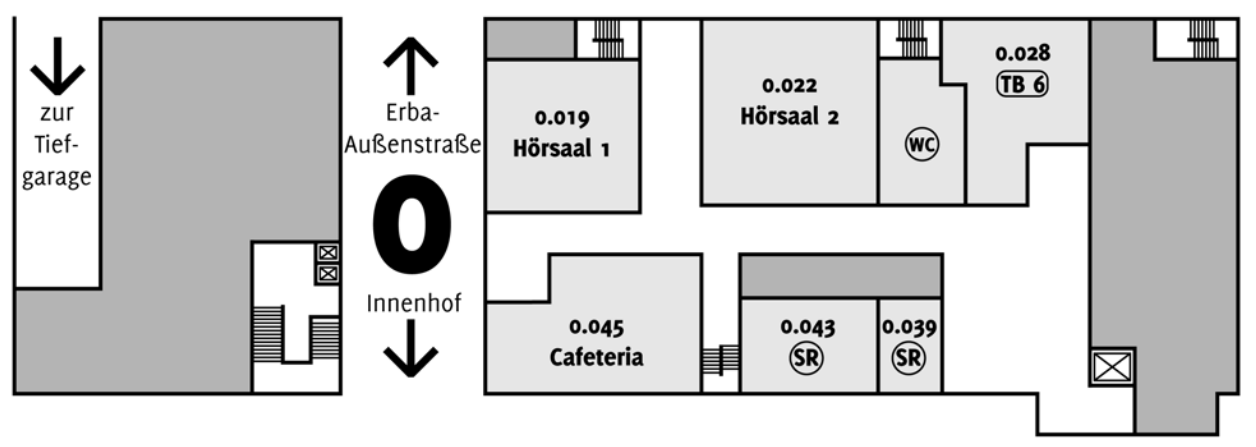
\includegraphics[width=.8\textheight, angle=90]{images/plan.png}
    };
\end{tikzpicture}
\end{center}

%
%
%Parking permits for visitors can also be obtained from three locations:
%\begin{enumerate}
%\item The Visitors Center, 109 Daniel Drive
%\item Parking Services, G01 Edgar Brown Union
%\item Clemson University Police, Memorial
%Stadium
%\end{enumerate}
%\section{Conference Banquet}
%The Banquet will be held 6:00 pm -- 7:30 pm in Calhoun Corners
%Restaurant located only 1/2 mile from the conference venues at
%103 Clemson Street
%Clemson, SC 29631
%(Phone: (864) 654-7490).
%
%%\includegraphics[scale=0.72]{restaurant_map.eps}
%
%The price, \underline{\bf not covered by organizers}, is \$23 and should
%be paid in cash upon arrival. The price does not include drinks.
%
%
%
%\section{Registration and Financial support} The
%conference is partially funded through NSF grant DMS-1201546.  Limited
%travel and lodging financial support will be available to the most
%attendees. However priority will be given to graduate students,
%post-docs and new Ph.D.s. Due to NSF regulations, we kindly ask all
%participants to register. If you have not already register please do so
%by visiting us at our web site:
%
%\url{http://www.devio.us/~ppunosevac/cdynsys/}
%
%
%Participants who are requesting financial support will also have to do
%vendor registration required by Clemson university as well as to submit
%expense report form with receipts.
%
%\section{Organizers}
%
%Martin Schmoll \url{<schmoll@clemson.edu>}
%
%Predrag Puno\v{s}evac \url{<ppunosev@aug.edu>}
\cleardoublepage
\newpage

\newpage
\section{Sponsors}
\begin{center}
\begin{tikzpicture}[yscale=-0.1, xscale=0.1, node distance=1mm,outer sep = 0pt]
\tikzset{grid/.style={gray,very thin,opacity=1}}
\tikzstyle{default}=[anchor=center,draw=red, fill=unibablueI]
    
%\draw[grid] (0,0) grid (10*\textwidth,10*\textheight);
\node[default] at (30,10) {
        
\includegraphics[width=.6\textwidth]{images/sterhard.pdf}
    };
\end{tikzpicture}
\end{center}


\end{document}